\subsection{Экспериментальные установки}
\begin{frame}
    \frametitle{$\text{e}^+\text{e}^-$ коллайдер KEKB}
    \begin{figure}
    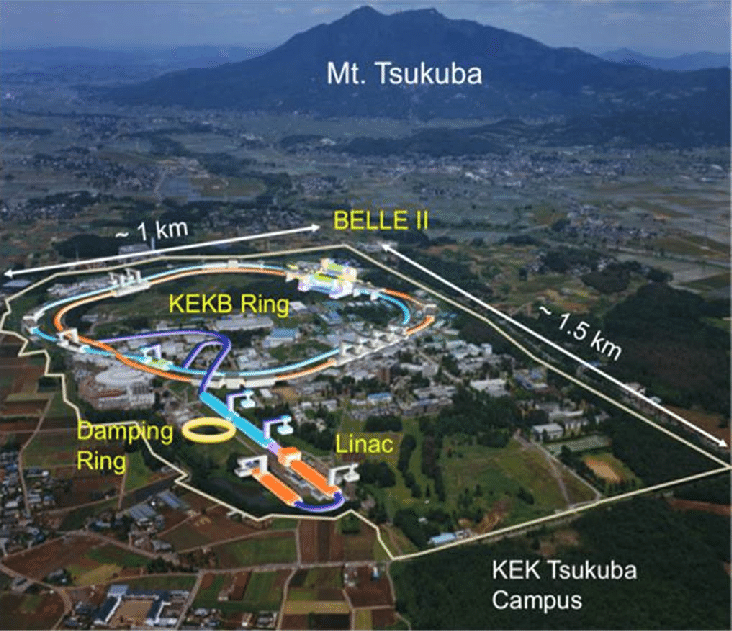
\includegraphics[
        height=0.8\textheight,
        width=\textwidth,
        keepaspectratio,
        ]{KEKB}
    \end{figure}
\end{frame}

\begin{frame}
    \frametitle{Детектор Белль}
    \begin{columns}
        \begin{column}{0.5\textwidth}
            \begin{figure}
            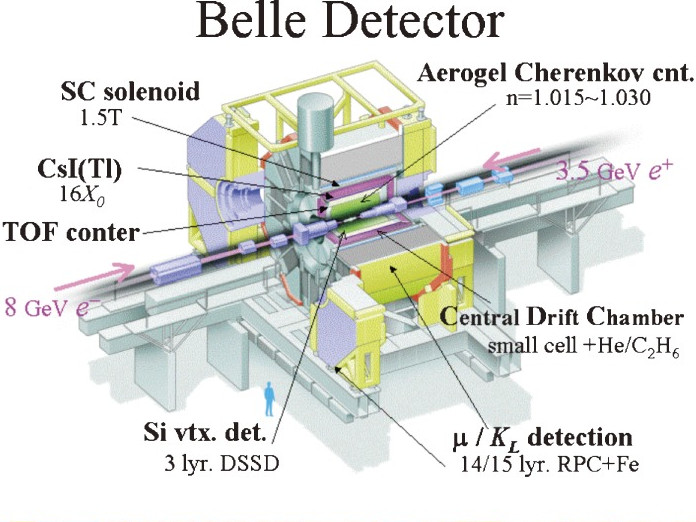
\includegraphics[
            height=0.9\textheight,
            width=\textwidth,
            keepaspectratio,
            ]{belle-side-view}
            \end{figure}
        \end{column}
        \begin{column}{0.5\textwidth}
            \begin{figure}
            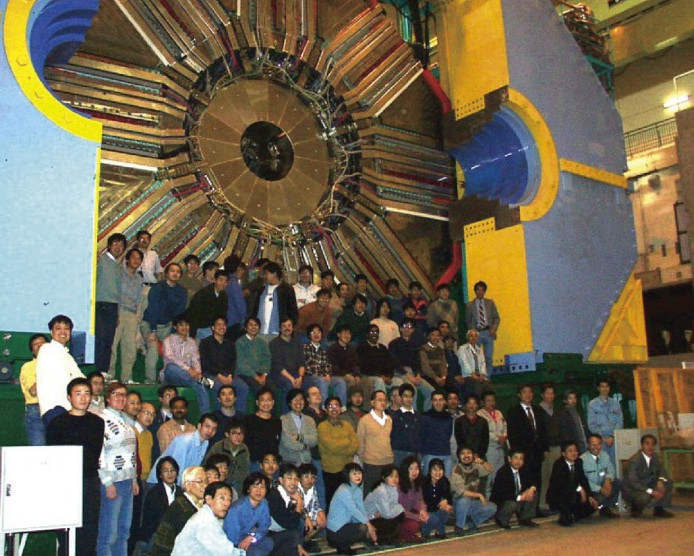
\includegraphics[
            height=0.9\textheight,
            width=\textwidth,
            keepaspectratio,
            ]{belle-collab}
            \end{figure}
        \end{column}
    \end{columns}
\end{frame}
%%%
\begin{frame}
    \frametitle{Дрейфовая камера}
    \begin{columns}
        \begin{column}{0.5\textwidth}
            \begin{figure}
            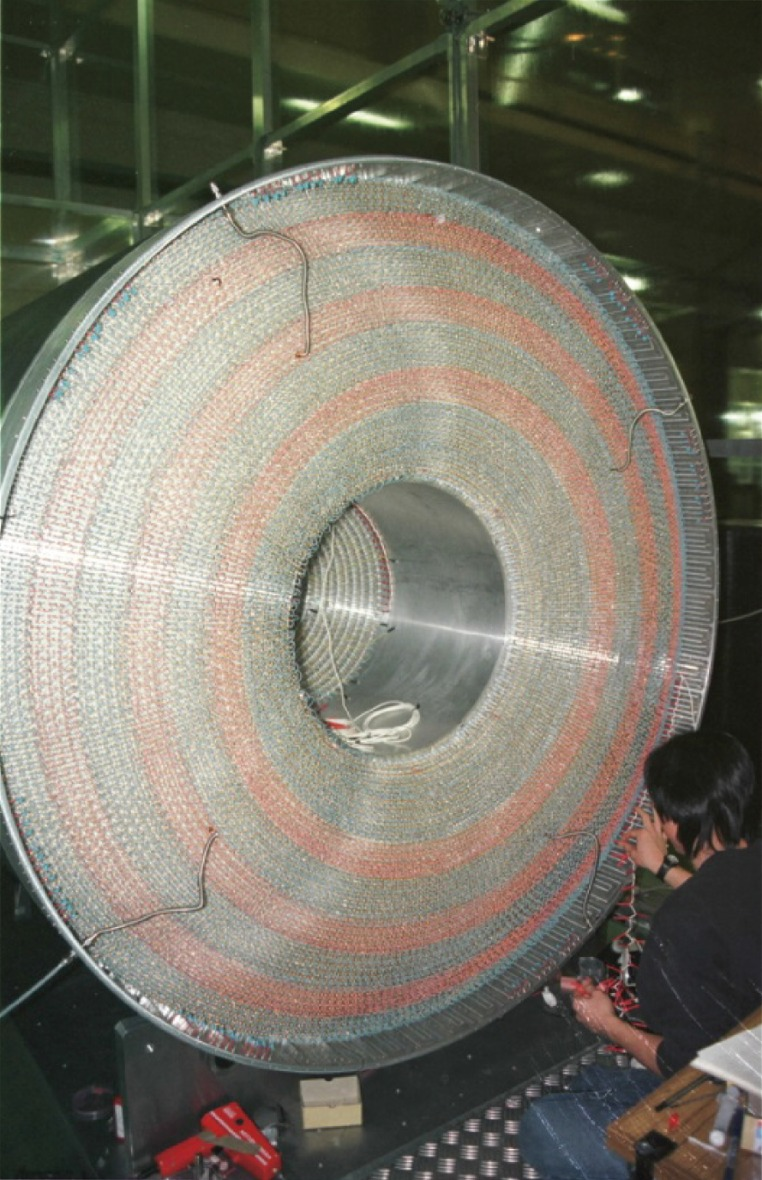
\includegraphics[
            height=0.7\textheight,
            width=0.9\textwidth,
            keepaspectratio,
            ]{belle-cdc}
            \end{figure}
        \end{column}
        \begin{column}{0.5\textwidth}
            \begin{figure}
            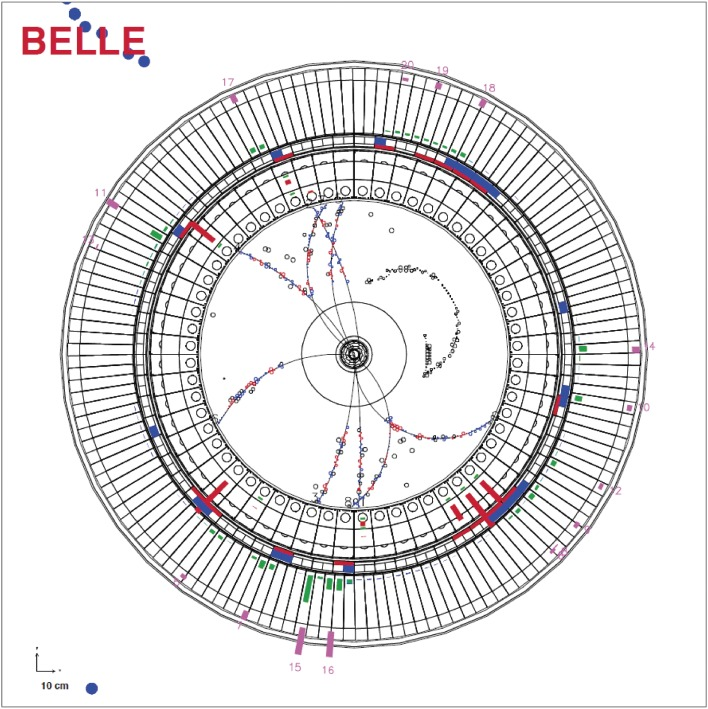
\includegraphics[
            height=0.9\textheight,
            width=0.85\textwidth,
            keepaspectratio,
            ]{belle-ed}
            \caption{Event display}
            \end{figure}
        \end{column}
    \end{columns}
\end{frame}
%%%
\begin{frame}
    \frametitle{Событие в детекторе}
    \begin{columns}
        \begin{column}{0.5\textwidth}
            \begin{figure}
            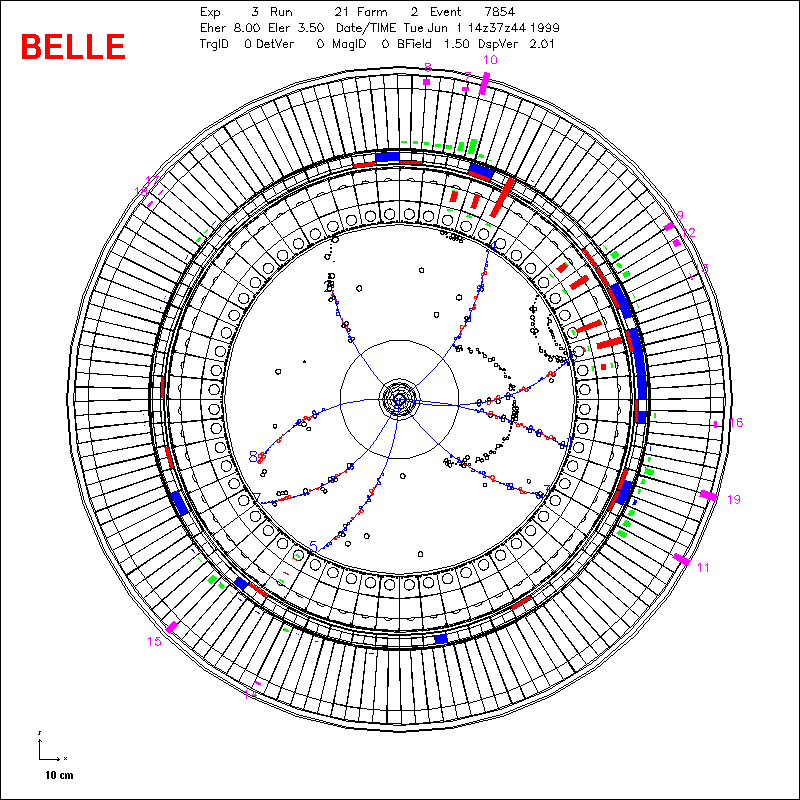
\includegraphics[
            height=0.95\textheight,
            width=0.9\textwidth,
            keepaspectratio,
            ]{belle-ed-xy}
            \caption{$\mathcal{XY}$-проекция}
            \end{figure}
        \end{column}
        \begin{column}{0.5\textwidth}
            \begin{figure}
            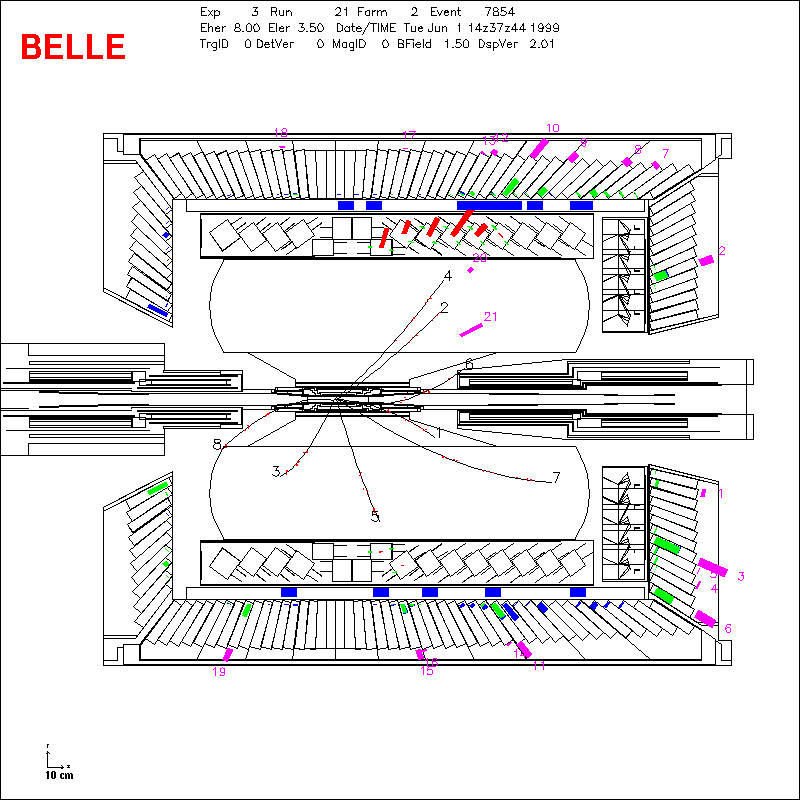
\includegraphics[
            height=0.95\textheight,
            width=0.9\textwidth,
            keepaspectratio,
            ]{belle-ed-yz}
            \caption{$\mathcal{YZ}$-проекция}
            \end{figure}
        \end{column}
    \end{columns}
\end{frame}
%%%
\begin{frame}
    \frametitle{Нарушение $\mathcal{T}$-симметрии}
    \begin{figure}
    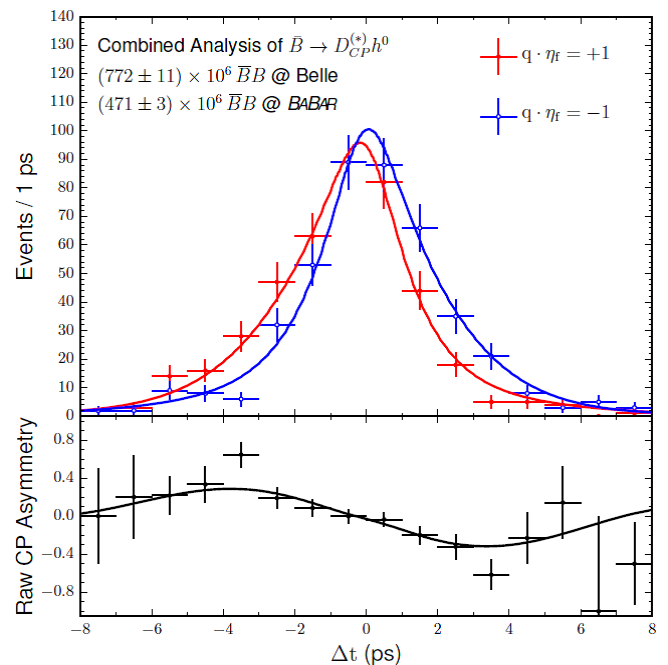
\includegraphics[
        height=0.8\textheight,
        width=\textwidth,
        keepaspectratio,
        ]{Tviolation}
    \end{figure}
\end{frame}
